%%%%%%%%%%%%%%%%%%%%%%%%%%%%%%%%%%%%%%%%%%%%%%%%
%% Compile: XeLaTeX BibTeX XeLaTeX XeLaTeX
%% Course Slides: LaTeX 4 Linguists -- LOT 2019, Amsterdam
%% Antonio Machicao y Priemer
%%%%%%%%%%%%%%%%%%%%%%%%%%%%%%%%%%%%%%%%%%%%%%%%

%\documentclass[a4paper,10pt, bibtotoc]{beamer}
\documentclass[a4paper,10pt,handout]{beamer}

%%%%%%%%%%%%%%%%%%%%%%%%%
%% PACKAGES & COMMANDS 
%%%%%%%%%%%%%%%%%%%%%%%%%

%%%%%%%%%%%%%%%%%%%%%%%%%%%%%%%%%%%%%%%%%%%%%%%%%%%%
%%%          MyP-Packages   2018.12.08    XeLaTeX
%%%%%%%%%%%%%%%%%%%%%%%%%%%%%%%%%%%%%%%%%%%%%%%%%%%%


%\usepackage[utf8]{inputenc} %XeLaTeX

%% For German texts
\usepackage[ngerman,english]{babel}

%% For English texts
%\usepackage[ngerman,english]{babel}

%% Captions numbered in Beamer 
\setbeamertemplate{caption}[numbered]

%% Change ''Abbildung'' into ''Abb.'' 
%% for: babel
	\renewcommand{\thefigure}{\arabic{figure}}
	\addto\captionsngerman{%
		\renewcommand{\figurename}{Abb.}%
	}
	\renewcommand{\figurename}{Abb.} 

%% Change ''Figure'' into ''Fig.'' 
%% for: babel
	\renewcommand{\thefigure}{\arabic{figure}}
	\addto\captionsenglish{%
		\renewcommand{\figurename}{Fig.}%
	}
%	\renewcommand{\figurename}{Fig.} %% << not needed? 


%% TIPA encoding needs options: T3 & T1
\usepackage[T3,T1]{fontenc}  %not needed in XeLaTeX (?)

%\usepackage{fontspec} % XeLaTeX: Problem: Libertine+Fontspec+TIPA

%% Font
\usepackage{lmodern}
%\usepackage{libertine} % XeLaTeX: Problem: Libertine+Fontspec+TIPA

%% Blind text: \blindtext \Blindtext \blindtext[5] \blindlist{itemize}[x] ...
\usepackage{blindtext}

%% ulem: Strike out
\usepackage[normalem]{ulem}  

%% graphicx: if gb4e is active PDFLaTeX does not accept files with underline. PDFLaTeX accepts files only with .jpg, .png, .pdf endings
\usepackage{graphicx}

%% Math symbols
\usepackage{amsmath}
\usepackage{amsfonts}
\usepackage{amssymb}
\usepackage{MnSymbol} 				% Meaning brackets 

%% Toggles
\usepackage{etoolbox}
	\newtoggle{handout}


%%%%%%%%%%%%%%%%%%%%%%%%%%%%%%%%%%%%%%%%%%%%%%%%%%%%
%%%         Tables & Lists & Columns            
%%%%%%%%%%%%%%%%%%%%%%%%%%%%%%%%%%%%%%%%%%%%%%%%%%%%

% Text in columns: \begin{multicols}{n} \columnbreak \end{multicols}
\usepackage{multicol}
%	\setlength{\columnsep}{.5cm}	

%% Tables with specified width
\usepackage{tabularx}

%% For complex tables
\usepackage{array}

%% For other tables
\usepackage{booktabs}

%% For more than one row in a table
\usepackage{multirow}

%% Special lists: itemize*
\usepackage{mdwlist}


%%%%%%%%%%%%%%%%%%%%%%%%%%%%%%%%%%%%%%%%%%%%%%%%%%%%
%%%          Coloured elements                  
%%%%%%%%%%%%%%%%%%%%%%%%%%%%%%%%%%%%%%%%%%%%%%%%%%%%
%Use xcolor before `gb4e'!
\usepackage{xcolor}


%%%%%%%%%%%%%%%%%%%%%%%%%%%%%%%%%%%%%%%%%%%%%%%%%%%%
%%%          Trees                               
%%%%%%%%%%%%%%%%%%%%%%%%%%%%%%%%%%%%%%%%%%%%%%%%%%%%
%% Forest must be loaded before `gb4e'
\usepackage{forest}
	
	%% Needed for the "actual forest version"
	\useforestlibrary{linguistics}
	\forestapplylibrarydefaults{linguistics}

%% Old forest version
%\usepackage{etex}		%For Forest bug
%\usepackage{../forestold}
	
	
%%%%%%%%%%%%%%%%%%%%%%%%%%%%%%%%%%%%%%%%%%%%%%%%%%%%
%%%          Venndiagram                         
%%%%%%%%%%%%%%%%%%%%%%%%%%%%%%%%%%%%%%%%%%%%%%%%%%%%
%% Package needed: tikz
\usepackage{venndiagram}


%%%%%%%%%%%%%%%%%%%%%%%%%%%%%%%%%%%%%%%%%%%%%%%%%%%%%
%%%%          Verbatim                            
%%%%%%%%%%%%%%%%%%%%%%%%%%%%%%%%%%%%%%%%%%%%%%%%%%%%%
%%`Listings' must be loaded before `gb4', use `verbatim' otherwise
\usepackage{listings}

\lstset{
	language=TeX,
	backgroundcolor=\color{lightgray},
	basicstyle={\footnotesize\ttfamily\color{blue}},
	showstringspaces=false,
	columns=flexible
}
\lstset{literate=%
	{Ö}{{\"O}}1
	{Ä}{{\"A}}1
	{Ü}{{\"U}}1
	{ß}{{\ss}}2
	{ü}{{\"u}}1
	{ä}{{\"a}}1
	{ö}{{\"o}}1
}

%\lstset{%frame=tb,
%	language=Perl,
%	aboveskip=3mm,
%	belowskip=3mm,
%	showstringspaces=false,
%	columns=flexible,
%	basicstyle={\small\ttfamily\color{blue}},
%	numbers=none,
%	%numberstyle=\tiny\color{gray},
%	extendedchars=false,
%	morekeywords={foo},
%	otherkeywords={\#\#},
%	%keywordstyle=\color{blau},
%	%commentstyle=\color{whiteblue},
%	%stringstyle=\color{mauve},
%	breaklines=true,
%	breakatwhitespace=true,
%	tabsize=3
%}


%%%%%%%%%%%%%%%%%%%%%%%%%%%%%%%%%%%%%%%%%%%%%%%%%%%%%
%%%%       Attribute Value Matrices               
%%%%%%%%%%%%%%%%%%%%%%%%%%%%%%%%%%%%%%%%%%%%%%%%%%%%%
\usepackage{../../texfiles-beamer/avm}
%%% Setting of avm (see LSP Guidelines)
	%	\avmfont{\sc}
	%	\avmvalfont{\it}
	\avmfont{\normalfont \scshape} 
	\avmvalfont{\normalfont \itshape} 
%% command to fontify the type values of an avm 
	\newcommand{\tpv}[1]{{\avmjvalfont #1}} 
%% command to fontify the type of an avm and avmspan it
	\newcommand{\tp}[1]{\avmspan{\tpv{#1}}}


%%%%%%%%%%%%%%%%%%%%%%%%%%%%%%%%%%%%%%%%%%%%%%%%%%%%
%%%          IPA                                 
%%%%%%%%%%%%%%%%%%%%%%%%%%%%%%%%%%%%%%%%%%%%%%%%%%%%
%\usepackage[noenc,safe]{tipa}	%in PDFLaTeX
\usepackage[safe]{tipa}	% in XeLaTeX


%%%%%%%%%%%%%%%%%%%%%%%%%%%%%%%%%%%%%%%%%%%%%%%%%%%%
%%%          Vowel diagram                       
%%%%%%%%%%%%%%%%%%%%%%%%%%%%%%%%%%%%%%%%%%%%%%%%%%%%
%\usepackage{vowel}


%%%%%%%%%%%%%%%%%%%%%%%%%%%%%%%%%%%%%%%%%%%%%%%%%%%%
%%%          Bibliography                        
%%%%%%%%%%%%%%%%%%%%%%%%%%%%%%%%%%%%%%%%%%%%%%%%%%%%
\usepackage{natbib}	
	\setcitestyle{notesep={:~}}


%%%%%%%%%%%%%%%%%%%%%%%%%%%%%%%%%%%%%%%%%%%%%%%%%%%%%
%%%%          Settings of the page                
%%%%%%%%%%%%%%%%%%%%%%%%%%%%%%%%%%%%%%%%%%%%%%%%%%%%%

%% (Vertical) Spacing
\usepackage{setspace}
%	\onehalfspacing

%% Space for abbreviations 'i.d.R'
\usepackage{xspace}

%% Margins % >> Option clash for beamer
%\usepackage[a4paper]{geometry} 	
%	\geometry{top=2.5cm, bottom=2.5cm, left=2.5cm, right=2.5cm}


%%%%%%%%%%%%%%%%%%%%%%%%%%%%%%%%%%%%%%%%%%%%%%%%%%%%%
%%%%          Margin notes                        
%%%%%%%%%%%%%%%%%%%%%%%%%%%%%%%%%%%%%%%%%%%%%%%%%%%%%
%% See definition in localcommands.sty, not working with Beamer class
%\usepackage{marginnote}


%%%%%%%%%%%%%%%%%%%%%%%%%%%%%%%%%%%%%%%%%%%%%%%%%%%%%%
%%%%%                Videos                        
%%%%%%%%%%%%%%%%%%%%%%%%%%%%%%%%%%%%%%%%%%%%%%%%%%%%%%
%%Embedding videos >> it does not work
%\usepackage{media9} 


%%%%%%%%%%%%%%%%%%%%%%%%%%%%%%%%%%%%%%%%%%%%%%%%%%%%
%%%          Hyperref & URL                      
%%%%%%%%%%%%%%%%%%%%%%%%%%%%%%%%%%%%%%%%%%%%%%%%%%%%

%\usepackage[hyphens]{url}
\usepackage{url}

%\usepackage{hyperref}

%\usepackage[
%	bookmarksnumbered, % For numbered bookmarks in PDF, not needed for Beamer class
%	hidelinks, %For links without colored borders
%	hyperfootnotes=false %If FNs takes you to the 1st page and not to the FN text
%	]{hyperref}


%%%%%%%%%%%%%%%%%%%%%%%%%%%%%%%%%%%%%%%%%%%%%%%%%%%%
%%%           Examples                           
%%%%%%%%%%%%%%%%%%%%%%%%%%%%%%%%%%%%%%%%%%%%%%%%%%%%

%%% Easy to use: 
%\usepackage{linguex}

%%% gb4e: more powerful than linguex, but with many bugs.
%%% Add gb4e as one of the last packages! 
%\usepackage{gb4e}

%% lsp-gb4eMyP: lsp-Variant of gb4e by MyP
\usepackage{../../texfiles-beamer/lsp-gb4eMyP}

%% (for lsp-gb4eMyP: to add additional information to the right of examples, uncomment the following line)
\usepackage{../../texfiles-beamer/jambox}
%	\jamwidth=2cm\relax 

%% (for lsp-gb4eMyP: if you want the source line of examples to be in italics, uncomment the following line)
% \def\exfont{\it}		


%%%%%%%%%%%%%%%%%%%%%%%%%%%%%%%%%%%%%%%%%%%%%%%%%%%%
%%%           Style Sheet HU                     %%%
%%%%%%%%%%%%%%%%%%%%%%%%%%%%%%%%%%%%%%%%%%%%%%%%%%%%
%% huberlin: Style sheet
\usepackage{../../texfiles-beamer/tex-styleHU/huberlin}

%%% Uni-Tuebingen: Style sheet
%\usepackage{../../texfiles-beamer/tex-styleHU/unituebingen}

%%%%%%%%%%%%%%%%%%%%%%%%%%%%%%%%%%%%%%%%%%%%%%%%%%%%
%%%           MyP-Commands  2018.12.08       
%%%%%%%%%%%%%%%%%%%%%%%%%%%%%%%%%%%%%%%%%%%%%%%%%%%%   


%%%%%%%%%%%%%%%%%%%%%%%%%%%%%%%%
% German quotation marks:
\newcommand{\gqq}[1]{\glqq{}#1\grqq{}}		%double
\newcommand{\gq}[1]{\glq{}#1\grq{}}			%simple


%%%%%%%%%%%%%%%%%%%%%%%%%%%%%%%%
% Abbreviations in German
% package needed: xspace
% Short space in German abbreviations: \,	
\newcommand{\dash}{\mbox{d.\,h.}\xspace}
\newcommand{\idR}{\mbox{i.\,d.\,R.}\xspace}
\newcommand{\su}{\mbox{s.\,u.}\xspace}
\newcommand{\ua}{\mbox{u.\,a.}\xspace}
\newcommand{\va}{\mbox{v.\,a.}\xspace}
\newcommand{\zB}{\mbox{z.\,B.}\xspace}
%\newcommand{\s}{s.~}
%not possibel: \dh --> d.\,h.


%%%%%%%%%%%%%%%%%%%%%%%%%%%%%%%%
%Abbreviations in English
\newcommand{\ao}{a.o.\ }	% among others
\newcommand{\cf}[1]{(cf.~#1)}	% confer = compare
\newcommand{\cfe}[1]{(cf.~(\ref{#1}))}	% compare + example
\newcommand{\ia}{i.a.}	% inter alia = among others
\newcommand{\ie}{i.e.~}	% id est = that is
\newcommand{\fe}{e.g.~}	% exempli gratia = for example
%not possible: \eg --> e.g.~
\newcommand{\vs}{vs.\ }	% versus
\newcommand{\wrt}{w.r.t.\ }	% with respect to


%%%%%%%%%%%%%%%%%%%%%%%%%%%%%%%%
% Dash:
\newcommand{\gs}[1]{--\,#1\,--}


%%%%%%%%%%%%%%%%%%%%%%%%%%%%%%%%
% Rightarrow with and without space
\def\ra{\ensuremath\rightarrow}			%without space
\def\ras{\ensuremath\rightarrow\ }		%with space
\def\la{\ensuremath\leftarrow}
\def\las{\ensuremath\leftarrow\ }


%%%%%%%%%%%%%%%%%%%%%%%%%%%%%%%%
%% X-bar notation

%% Notation with primes (not emphasized): \xprime{X}
\newcommand{\xprime}[1]{#1$^{\prime}$}
\newcommand{\xxprime}[1]{#1$^{\prime\prime}$}
\newcommand{\xxxprime}[1]{#1$^{\prime\prime\prime}$}

%% Notation with primes (emphasized): \exbar{X}
\newcommand{\exprime}[1]{\emph{#1}$^{\prime}$}
\newcommand{\exxprime}[1]{\emph{#1}$^{\prime\prime}$}
\newcommand{\exxxprime}[1]{\emph{#1}$^{\prime\prime\prime}$}

% Notation with zero and max (not emphasized): \xbar{X}
\newcommand{\xzero}[1]{#1$^{0}$}
\newcommand{\maxbar}[1]{#1$^{\textsc{max}}$}

% Notation with zero and max (emphasized): \xbar{X}
\newcommand{\ezerobar}[1]{\emph{#1}$^{0}$}
\newcommand{\emaxbar}[1]{\emph{#1}$^{\textsc{max}}$}

%% Notation with bars (already implemented in gb4e):
% \obar{X}, \ibar{X}, \iibar{X}, \mbar{X} %Problems with \mbar!
% $\overline{}$
%
%% Without gb4e:
\newcommand{\overbar}[1]{\mkern 1.5mu\overline{\mkern-1.5mu#1\mkern-1.5mu}\mkern 1.5mu}
%
%%% OR:
%\newcommand{\ibar}[1]{$\overline{\textrm{#1}}$}
%\newcommand{\iibar}[1]{$\overline{\overline{\textrm{#1}}}$}
%% (emphasized):
\newcommand{\eibar}[1]{$\overline{#1}$}
\newcommand{\eiibar}[1]{\overline{$\overline{#1}}$}


%%%%%%%%%%%%%%%%%%%%%%%%%%%%%%%%
%% Subscript & Superscript: no italics inside math mode
\newcommand{\down}[1]{\textsubscript{#1}}
\newcommand{\downm}[1]{_{\textrm{#1}}}

\newcommand{\up}[1]{\textsuperscript{#1}}
\newcommand{\upm}[1]{^{\textrm{#1}}}


%%%%%%%%%%%%%%%%%%%%%%%%%%%%%%%%
%% Small caps subscripts
\newcommand{\scdown}[1]{\textsubscript{\textsc{#1}}}


%%%%%%%%%%%%%%%%%%%%%%%%%%%%%%%%%
%%% Shorter Underline
%\DeclareTextCommand{\_}{T1}{\leavevmode \kern.06em\vbox{\hrule width.4em}}


%%%%%%%%%%%%%%%%%%%%%%%%%%%%%%%%
%% Object- and Meta-language marking:
%\newcommand{\obj}[1]{\glqq{}#1\grqq{}}		%German double quotes
%\newcommand{\obj}[1]{``#1''}					  %English double quotes
\newcommand{\obj}[1]{\emph{#1}}                 %Emphasising
\newcommand{\term}[1]{\textsc{#1}}              %for abbreviated terminology


%%%%%%%%%%%%%%%%%%%%%%%%%%%%%%%%
% Size:
\newcommand{\size}[1]{{\footnotesize #1}}	% f.e. resize citations


%%%%%%%%%%%%%%%%%%%%%%%%%%%%%%%%
%% for LaTeX terminology: package names, environments, commands
\newcommand{\ltxterm}[1]{{\footnotesize \texttt{#1}}}
\newcommand{\ltxpack}[1]{{\footnotesize \texttt{#1}}}


%%%%%%%%%%%%%%%%%%%%%%%%%%%%%%%%
% Short cuts (<STRG + ALT>):
%\newcommand{\short}[1]{\texttt{\textsc{#1}}}		%Emphasising
\newcommand{\short}[1]{$\langle$\texttt{\textsc{#1}}$\rangle$}		%Emphasising


%%%%%%%%%%%%%%%%%%%%%%%%%%%%%%%%
% Writing text with colour:
% package needed: xcolor
% Command \alert{} in Beamer >> red
\newcommand{\blue}[1]{\textcolor{blue}{#1}}
\newcommand{\green}[1]{\textcolor{green}{#1}}
\newcommand{\red}[1]{\textcolor{red}{#1}}


%%%%%%%%%%%%%%%%%%%%%%%%%%%%%%%%
%% Marking text with colour: 
%%% package needed: color
\newcommand{\clrr}[1]{\colorbox{red}{#1}}
\newcommand{\clry}[1]{\colorbox{yellow}{#1}}


%%%%%%%%%%%%%%%%%%%%%%%%%%%%%%%%
%% Semantic types (<e,t>), features, variables and graphemes in angled brackets 

%%% types and variables, in math mode: angled brackets + italics + no space
%\newcommand{\type}[1]{$<#1>$}

%%% OR more correctly: 
%%% Types and Variables: chevrons! + text in math mode (italics + no space)
\newcommand{\type}[1]{$\langle #1 \rangle$} %% In Math Mode, only single types
\newcommand{\typem}[1]{\langle #1 \rangle } %% Mathmode extra, complex types

%%% Features and Graphemes: chevrons! + normal font
\newcommand{\ab}[1]{$\langle$#1$\rangle$} %% no italics
\newcommand{\abe}[1]{$\langle$\emph{#1}$\rangle$} %% italics


%%%%%%%%%%%%%%%%%%%%%%%%%%%%%%%%
%% Function symbol in Beamer Class!
%% italics and serif
\newcommand{\func}{\emph{\textrm{f}}}
\newcommand{\gunc}{\emph{\textrm{g}}}
\newcommand{\chiF}[1]{\chi _{\textrm{#1}}} 


%%%%%%%%%%%%%%%%%%%%%%%%%%%%%%%%
%% HPSG: Features and Values!
\newcommand{\wert}[1]{\emph{#1}}		%Values & Types
\newcommand{\val}[1]{\emph{#1}}		%Values & Types
\newcommand{\feat}[1]{\textsc{#1}}	%Features


%%%%%%%%%%%%%%%%%%%%%%%%%%%%%%%%
%% (Syntactic) Trees
% package needed: forest
%
%%% Setting for simple trees
%\forestset{
%	sn edges/.style={for tree={parent anchor=south, child anchor=north}}
%}

%%% Setting for complex trees
%\forestset{
%	sn edges/.style={for tree={parent anchor=south, child anchor=north,align=center,base=bottom,where n children=0{tier=word,inner xsep=0pt,outer sep=0pt}{}}}, 
%background tree/.style={for tree={text opacity=0.2,draw opacity=0.2,edge={draw opacity=0.2}}}
%}
%
%\newcommand\HideWd[1]{%
%	\makebox[0pt]{#1}%
%}


%%%%%%%%%%%%%%%%%%%%%%%%%%%%%%%%
%% Outputbox
\newcommand{\outputbox}[1]{\noindent\fbox{\parbox[t][][t]{0.98\linewidth}{#1}}\vspace{0.5em}}


%%%%%%%%%%%%%%%%%%%%%%%%%%%%%%%%
% Margin notes: \myp{NOTE}
% package needed: marginnote
\renewcommand{\marginfont}{\singlespacing}
\renewcommand{\marginfont}{\footnotesize}
\renewcommand{\marginfont}{\color{black}}

\newcommand{\myp}[1]{%
	\marginnote{%
		\begin{spacing}{1}
			\vspace{-\baselineskip}%
			\color{red}\scriptsize#1
		\end{spacing}
	}
}


%%%%%%%%%%%%%%%%%%%%%%%%%%%%%%%%
%% Corpora & Grammmars
\newcommand{\DWDS}[1]{DWDS\nocite{DWDS}: #1}
 
\newcommand{\CREA}{\citetext{CREA \citeyear{CREA}}}
\newcommand{\CREAA}{\citetext{CREA \citeyear{CREAA}}}
\newcommand{\CORPES}{\citetext{CORPES \citeyear{CORPES}}}

\newcommand{\DECOW}{\citetext{DECOW \citeyear{SchaeferR15a}}}
\newcommand{\ESCOW}{\citetext{ESCOW \citeyear{SchaeferR&Co12a}}}

\newcommand{\RAEa}[1]{RAE, \citeyear[#1]{RAE10a}}
\newcommand{\RAEb}[1]{RAE, \citeyear[#1]{RAE10b}}


%%%%%%%%%%%%%%%%%%%%%%%%%%%%%%%%
%% Literature and Appendix
\newcommand{\backupbegin}{
	\newcounter{finalframe}
	\setcounter{finalframe}{\value{framenumber}}
}
\newcommand{\backupend}{
	\setcounter{framenumber}{\value{finalframe}}
}


%%%%%%%%%%%%%%%%%%%%%%%%%%%%%%%%%%%%%%%%%%%%%%%%%%%%
%%%          Useful commands                    
%%%%%%%%%%%%%%%%%%%%%%%%%%%%%%%%%%%%%%%%%%%%%%%%%%%%


%%%%%%%%%%%%%%%%%%%%%%%%%%%%%%%%%%%
%%%%%%%%%%%%%%%%%%%%%%%%%%%%%%%%%%%
%\section{XY}
%%\frame{
%%\begin{multicols}{2}
%%\frametitle{~}
%%	\tableofcontents[currentsection]
%%\end{multicols}
%%}
%%%%%%%%%%%%%%%%%%%%%%%%%%%%%%%%%%%
%
%\begin{frame}{XY}
%
%\begin{itemize}
%	\item XY
%\end{itemize}
%
%\end{frame}


%%%%%%%%%%%%%%%%%%%%%%%%%%%%%%%%%%%
%%%%%%%%%%%%%%%%%%%%%%%%%%%%%%%%%%%
%\iftoggle{handout}{
%	
%%%%%%%%%%%%%%%%%%%%%%%%%%%%%%%%%%%
%\begin{frame}
%%\frametitle{Bücher \& Artikel}
%	
%Test Toggle ON
%	
%\end{frame}
%
%}
%%% END handout true 
%%% BEGIN handout false
%{
%%%%%%%%%%%%%%%%%%%%%%%%%%%%%%%%%%%
%
%%% EMPTY
%
%}%% END HO-Toggle
%%%%%%%%%%%%%%%%%%%%%%%%%%%%%%%%%%%


%%%%%%%%%%%%%%%%%%%%%
%% COMMENTING BLOCKS
% \if0    \fi 

%%%%%%%%%%%%%%%%%%%%%
%% FOR ITEMS:
%\begin{itemize}
%  \item<2-> from point 2
%  \item<3-> from point 3 
%  \item<4-> from point 4 
%\end{itemize}
%
% or: \onslide<2->
% or: \visible<overlay specification>{text}
% or: \only<overlay specification>{text}
% or: \pause

%%%%%%%%%%%%%%%%%%%%%
%% JAMBOX FOR EXAMPLES:
%\ea 
%\settowidth\jamwidth{ Test} 
%Die Studierenden, die weitgehend von Stipendien leben, erhalten einen Mietzuschuss. 
%\jambox{Test}
%\z 

%%%%%%%%%%%%%%%%%%%%%
%% VERTICAL SPACE:
% \vspace{.5cm}
% \vfill

%%%%%%%%%%%%%%%%%%%%%
% RED MARKING OF TEXT:
%\alert{bis spätestens Mittwoch, 18 Uhr}

%%%%%%%%%%%%%%%%%%%%%
%% RESCALE BIG TABLES:
%\scalebox{0.8}{
%For Big Tables
%}

%%%%%%%%%%%%%%%%%%%%%
%% BLOCKS:
%\begin{alertblock}{Title}
%Text
%\end{alertblock}
%
%\begin{block}{Title}
%Text
%\end{block}
%
%\begin{exampleblock}{Title}
%Text
%\end{exampleblock}

%%%%%%%%%%%%%%%%%%%%%
%% MINIPAGE:
%\begin{minipage}[ÄUSSERE POSITION][HÖHE][INNERE POSITION]{BREITE}
%	Beispieltext
%\end{minipage}
%
%% MINIPAGE EXAMPLE:
%\begin{minipage}[b][][c]{.45\textwidth}
%	\onslide<2->
%	\begin{figure}
%		\centering
%		\includegraphics[scale=.1]{../material/Vierecke-Fee1}
%		\caption{Vierecke 1}
%	\end{figure}
%\end{minipage}
%%
%\begin{minipage}[b][][c]{.45\textwidth}
%	\onslide<3->
%	\begin{figure}
%		\centering
%			\includegraphics[scale=.1]{../material/Vierecke-Fee2}
%		\caption{Vierecke 2}
%	\end{figure}
%\end{minipage}	
%%

%%%%%%%%%%%%%%%%%%%%%
%% VIDEO:
%\begin{frame}
%\frametitle{Vor fast 54 Jahren in Berlin \dots}
%
%\begin{center}
%	\includemedia[
%	width=0.9\linewidth,height=0.506\linewidth,
%	activate=pageopen,
%	flashvars={
%		modestbranding=1 % no YT logo in control bar
%		&autohide=1 % controlbar autohide
%		&showinfo=0 % no title and other info before start
%		&rel=0 % no related videos after end
%		&playsinline=0
%		&start=28.5
%	}
%	]{}{http://www.youtube.com/v/NaZ3onbUrew}
%\end{center}
%
%\end{frame}


%%%%%%%%%%%%%%%%%%%%%%%%%%%%%%%%%%%%%%%%%%%%%%%%%%%%
%%%          NOTES: To Check                    
%%%%%%%%%%%%%%%%%%%%%%%%%%%%%%%%%%%%%%%%%%%%%%%%%%%% 

% Do I use ``'' or \emph{•} for object language?



%%%%%%%%%%%%%%%%%%%%%%%%%%%%%%%%%%%%%%%%%%%%%%%%%%%%
%%%             Preamble's End                   
%%%%%%%%%%%%%%%%%%%%%%%%%%%%%%%%%%%%%%%%%%%%%%%%%%%% 

\begin{document}

\togglefalse{handout}
%\toggletrue{handout}

%%%%%%%%%%%%%%%%%%%%%%%%%%%%%%%%%%%%%%%%%%%%%%%%
%% Compile the master file!
%% 		Slides: Antonio Machicao y Priemer
%% 		Course: Wissenschaftliches Arbeiten
%%%%%%%%%%%%%%%%%%%%%%%%%%%%%%%%%%%%%%%%%%%%%%%%


%%%%%%%%%%%%%%%%%%%%%%%%%%%%%%%%%%%%%%%%%%%%%%%%%%%%
%%%             Metadata                         
%%%%%%%%%%%%%%%%%%%%%%%%%%%%%%%%%%%%%%%%%%%%%%%%%%%%  

\title{
	\LaTeX\ for Linguists
}

\subtitle{\LaTeX\ 3: Graphics, tables \& floats}

\author[aMyP]{
	{\small Sebastian Nordhoff \& Antonio Machicao y Priemer}
	\\
	{\footnotesize \url{www.linguistik.hu-berlin.de/staff/amyp}}
	%	\\
	%	{\footnotesize \href{mailto:mapriema@hu-berlin.de}{mapriema@hu-berlin.de}}
}

\institute{LOT 2019, Amsterdam}

%\date{ }

%\publishers{\textbf{6. linguistischer Methodenworkshop \\ Humboldt-Universität zu Berlin}}

%\hyphenation{nobreak}


%%%%%%%%%%%%%%%%%%%%%%%%%%%%%%%%%%%%%%%%%%%%%%%%%%%%
%%%             Preamble's End                   
%%%%%%%%%%%%%%%%%%%%%%%%%%%%%%%%%%%%%%%%%%%%%%%%%%%%      


%%%%%%%%%%%%%%%%%%%%%%%%%%%%%%%%%%%
%%%%%%%%%%%%%%%%%%%%%%%%%%%%%%%%%%%    
%% Title slide 
\begin{frame}
  \HUtitle
\end{frame}


%% Contents slide
\frame{
\begin{multicols}{2}
	\frametitle{Contents}
%	\tableofcontents[hideallsubsections]
	\tableofcontents
	%[pausesections]
\end{multicols}
	}


%%%%%%%%%%%%%%%%%%%%%%%%%%%%%%%%%%%%
%%%%%%%%%%%%%%%%%%%%%%%%%%%%%%%%%%%%
%% Extra literature

\nocite{Freitag&MyP15a}
\nocite{Knuth1986}
\nocite{Kopka94a}
\nocite{MyP17c}
\nocite{MyP&Kerkhof16a}
	
%%%%%%%%%%%%%%%%%%%%%%%%%%%%%%%%%%%%
%%%%%%%%%%%%%%%%%%%%%%%%%%%%%%%%%%%%


%%%%%%%%%%%%%%%%%%%%%%%%%%%%%%%%%%%%%
%%%%%%%%%%%%%%%%%%%%%%%%%%%%%%%%%%%%%
%%%% Basic literature for these slides
%
%\begin{frame}
%\frametitle{Grundlage \& empfohlene Lektüre}
%
%\dots basierend auf \citet{Freitag&MyP15a} und auf \citet{MyP&Kerkhof16a}\\
%\ras \href{https://www.researchgate.net/publication/279514740_LATEX-Einfuhrung_fur_Linguisten}{LINK}
%
%
%\nocite{Kopka94a}
%
%\end{frame}


%%%%%%%%%%%%%%%%%%%%%%%%%%%%%%%%%%
%%%%%%%%%%%%%%%%%%%%%%%%%%%%%%%%%%
\section{Graphics}
\frame{
\begin{multicols}{2}
\frametitle{~}
	\tableofcontents[currentsection,hideallsubsections]
\end{multicols}
}
%%%%%%%%%%%%%%%%%%%%%%%%%%%%%%%%%%


%%%%%%%%%%%%%%%%%%%%%%%%%%%%%%%%%%
%%%%%%%%%%%%%%%%%%%%%%%%%%%%%%%%%%
\subsection{Including a graphic}
%\frame{
%	%\frametitle{~}
%	\begin{multicols}{2}
%		\tableofcontents[currentsection,hideallsubsections]
%	\end{multicols}
%}
%%%%%%%%%%%%%%%%%%%%%%%%%%%%%%%%%%

\begin{frame}[fragile]
\frametitle{Including a graphic}


\begin{itemize}
	\item Load the \textbf{package} \ltxterm{graphicx}: \lstinline|\usepackage{graphicx}|
	
%\begin{lstlisting}
%\usepackage{graphicx}
%\end{lstlisting}
	
	\item To include the graphic, use the following command (\textbf{file ending}, \ie \ltxpack{.pdf}, doesn't need to be added) :
	
\begin{lstlisting}
\includegraphics[size of graphic]{path/name of graphic}  
\end{lstlisting}

\end{itemize}

\pause
	
%\textbf{Example:}


\includegraphics{../../texfiles-beamer/tex-material/WissArb-latex/LaTeX-flowchart-1.pdf}   

\begin{lstlisting}
\includegraphics{LaTeX-flowchart-1.pdf}    
\end{lstlisting}


\end{frame}

%%%%%%%%%%%%%%%%%%%%%%%%%%%%%%%%%%
%%%%%%%%%%%%%%%%%%%%%%%%%%%%%%%%%%
\subsection{Rescaling the graphic}
%\frame{
%	%\frametitle{~}
%	\begin{multicols}{2}
%		\tableofcontents[currentsection,hideallsubsections]
%	\end{multicols}
%}
%%%%%%%%%%%%%%%%%%%%%%%%%%%%%%%%%%%
\begin{frame}[fragile]
\frametitle{Rescaling the graphic}

Rescaling \textbf{relative} to the \textbf{original size} with the option \lstinline|scale| (\lstinline|scale=0.5| $=$ 50\,\% of the original size)

\begin{lstlisting}
\includegraphics[scale=0.5]{LaTeX-flowchart-1.pdf}  
\end{lstlisting}

\includegraphics[scale=0.5]{../../texfiles-beamer/tex-material/WissArb-latex/LaTeX-flowchart-1.pdf}


\end{frame}


%%%%%%%%%%%%%%%%%%%%%%%%%%%%%%%%%%
\begin{frame}[fragile]
\frametitle{Rescaling the graphic}

Rescaling with \textbf{absolute specification} 


\begin{lstlisting}
\includegraphics[width=5cm]{LaTeX-flowchart-1.pdf}
\includegraphics[height=5cm]{LaTeX-flowchart-1.pdf}
\end{lstlisting}

\includegraphics[width=5cm]{../../texfiles-beamer/tex-material/WissArb-latex/LaTeX-flowchart-1}

Rescaling \textbf{relative} to the \textbf{document size}

\begin{lstlisting}
\includegraphics[width=\linewidth]{LaTeX-flowchart-1.pdf}  
\includegraphics[width=.2\linewidth]{LaTeX-flowchart-1.pdf}
\includegraphics[width=.2\textwidth]{LaTeX-flowchart-1.pdf}
\end{lstlisting}

%\includegraphics[width=.2\textwidth]{../../texfiles-beamer/tex-material/WissArb-latex/LaTeX-flowchart-1.pdf}

\includegraphics[width=.2\linewidth]{../../texfiles-beamer/tex-material/WissArb-latex/LaTeX-flowchart-1}
\end{frame}


%%%%%%%%%%%%%%%%%%%%%%%%%%%%%%%%%%
%%%%%%%%%%%%%%%%%%%%%%%%%%%%%%%%%%
\subsection{Formats and paths}
%\frame{
%	%\frametitle{~}
%	\begin{multicols}{2}
%		\tableofcontents[currentsection,hideallsubsections]
%	\end{multicols}
%}
%%%%%%%%%%%%%%%%%%%%%%%%%%%%%%%%%%

\begin{frame}[fragile]
\frametitle{Formats and paths}

\begin{itemize}
\item The following \textbf{formats} can be used with Xe\LaTeX\ and PDF\LaTeX :
	\begin{itemize}
	\item \ltxterm{.pdf} (vector graphics)
	\item \ltxterm{.png} (raster graphics)
	\item \ltxterm{.jpg} (raster graphics)
	\item \ltxterm{.eps} (vector graphics) (in Xe\LaTeX\ or with \ltxterm{epstopdf} package in PDF\LaTeX )
	\end{itemize}

\pause 

\item You must specify the place where you have saved the graphic \textbf{starting from the location of your \ltxterm{.tex}-file}.

\begin{enumerate}
	\item Graphic and  \ltxterm{.tex}-file are in the same folder:	
	
	\lstinline|\includegraphics{LaTeX-flowchart-1}|
	
	\item Graphic is in a folder \texttt{graphics}. This folder is in the same folder as your  \ltxterm{.tex}-file: 
	
	\lstinline|\includegraphics{graphics/LaTeX-flowchart-1}|
	
	\item \ltxterm{.tex}-file is in a folder. This folder and your graphic are in the same folder: 
	
	\lstinline|\includegraphics{../LaTeX-flowchart-1}|
\end{enumerate}

\end{itemize}

\end{frame}


%%%%%%%%%%%%%%%%%%%%%%%%%%%%%%%%%
\begin{frame}[fragile]
\frametitle{Exercise}

Go to \url{https://github.com/langsci/latex4linguists/blob/master/2-1.md}\\
and follow the instructions of the first \textbf{three blocks} in your \texttt{.tex} file.

\end{frame}


%%%%%%%%%%%%%%%%%%%%%%%%%%%%%%%%%%
%%%%%%%%%%%%%%%%%%%%%%%%%%%%%%%%%%
\section{Tables}
\frame{
%\frametitle{~}
\begin{multicols}{2}
	\tableofcontents[currentsection,hideallsubsections]
\end{multicols}
}
%%%%%%%%%%%%%%%%%%%%%%%%%%%%%%%%%%

\begin{frame}[fragile]
\frametitle{Tables}

\begin{itemize}
	\item \textbf{environment} for tables: \ltxterm{tabular} 
	\item optional argument for \textbf{position} of table
	\item obligatory argument for \textbf{layout} inside a column
	\item separation of table cells: \& 
	\item End of a row: \textbackslash\textbackslash 
\end{itemize}

%\begin{lstlisting}
%\begin{tabular}[position]{layout}
%...    
%\end{tabular}
%\end{lstlisting}

\pause 

\textbf{Example:}

\begin{multicols}{2}
	
%{\scriptsize
\begin{lstlisting}
sample text	
\begin{tabular}[t]{l|c|r}
0001 & 002 & 03 \\
\hline
0A & 000B & 00C \\
\hline
00i  & 0ii  & 000iii  \\
\end{tabular}
\end{lstlisting}
%}
	
	\columnbreak
	
	%\scalebox{.8}{
sample text	
	\begin{tabular}[t]{l|c|r}
%		\hline
		0001 & 002 & 03 \\
		\hline
		0A & 000B & 00C \\
		\hline
		00i  & 0ii  & 000iii  \\
%		\hline
	\end{tabular}
	%}
\end{multicols}

\end{frame}


%%%%%%%%%%%%%%%%%%%%%%%%%%%%%%%%%%%
%\begin{frame}[fragile]
%
%\begin{itemize}
%	\item possible values for \textbf{option}: \ltxterm{t} (top, (\ref{ex:TabTop})), \ltxterm{b} (bottom, (\ref{ex:TabBot})), or \ltxterm{c} (center, (\ref{ex:TabCent})) -- Default: \ltxterm{c}
%	
%	\begin{exe}
%		\ex\label{ex:TabTop} \ltxterm{t}:		
%		sample text	
%		\begin{tabular}[t]{l|c|r}
%			%		\hline
%			0001 & 002 & 03 \\
%			\hline
%			0A & 000B & 00C \\
%			\hline
%			00i  & 0ii  & 000iii  \\
%			%		\hline
%		\end{tabular}
%	
%\pause 
%	
%		\ex\label{ex:TabBot}  \ltxterm{b}:	
%		sample text	
%		\begin{tabular}[b]{l|c|r}
%			%		\hline
%			0001 & 002 & 03 \\
%			\hline
%			0A & 000B & 00C \\
%			\hline
%			00i  & 0ii  & 000iii  \\
%			%		\hline
%		\end{tabular}
%
%\pause 
%
%		\ex\label{ex:TabCent}  \ltxterm{c}:
%		sample text	
%		\begin{tabular}[c]{l|c|r}
%			%		\hline
%			0001 & 002 & 03 \\
%			\hline
%			0A & 000B & 00C \\
%			\hline
%			00i  & 0ii  & 000iii  \\
%			%		\hline
%		\end{tabular}
%	\end{exe}
%\end{itemize}
%
%\end{frame}


%%%%%%%%%%%%%%%%%%%%%%%%%%%%%%%%%%%
%\begin{frame}[fragile]
%%\frametitle{Tabellen}
%
%Die Option \textbf{Position} kann die Werte \ltxterm{t} (top), \ltxterm{c} (center), oder \ltxterm{b} (bottom) annehmen. 
%Diese Positionswerte geben die \textbf{vertikale Positionierung der gesamten Tabelle in Bezug zur aktuellen Zeile} (zur zuletzt geschriebenen Zeile), die Default-Einstellung ist in diesem Fall \ltxterm{center}.
%
%\begin{multicols}{2}
%
%Code für \textbf{top}:
%
%\columnbreak
%
%{\scriptsize
%	\begin{lstlisting}
%	Hier ist die aktuelle Zeile
%	\begin{tabular}[t]{l|c|r}
%	Zelle 01 & Zelle 02 & Zelle 03 \\
%	\hline
%	Zelle A & Zelle B & Zelle C \\
%	\hline
%	Zelle  & Zelle  & Zelle  \\
%	\end{tabular}
%	\end{lstlisting}
%}
%
%\end{multicols}
%
%Hier ist die aktuelle Zeile	
%\begin{tabular}[t]{l|c|r}
%Zelle 01 & Zelle 02 & Zelle 03 \\
%\hline
%Zelle A & Zelle B & Zelle C \\
%\hline
%Zelle  & Zelle  & Zelle  \\
%\end{tabular}
%
%\end{frame}
%
%
%%%%%%%%%%%%%%%%%%%%%%%%%%%%%%%%%%%
%\begin{frame}[fragile]
%%\frametitle{Tabellen}
%
%\begin{multicols}{2}
%
%Code für \textbf{bottom}:
%
%\columnbreak
%
%{\tiny
%\begin{lstlisting}
%Hier ist die aktuelle Zeile
%\begin{tabular}[b]{l|c|r}
%Zelle 01 & Zelle 02 & Zelle 03 \\
%\hline
%Zelle A & Zelle B & Zelle C \\
%\hline
%Zelle  & Zelle  & Zelle  \\
%\end{tabular}
%\end{lstlisting}
%}
%
%\end{multicols}
%
%Hier ist die aktuelle Zeile	
%\begin{tabular}[b]{l|c|r}
%Zelle 01 & Zelle 02 & Zelle 03 \\
%\hline
%Zelle A & Zelle B & Zelle C \\
%\hline
%Zelle  & Zelle  & Zelle  \\
%\end{tabular}
%
%
%\pause 
%
%
%\begin{multicols}{2}
%
%Code für \textbf{center}:
%
%\columnbreak
%
%{\tiny
%\begin{lstlisting}
%Hier ist die aktuelle Zeile
%\begin{tabular}[c]{l|c|r}
%Zelle 01 & Zelle 02 & Zelle 03 \\
%\hline
%Zelle A & Zelle B & Zelle C \\
%\hline
%Zelle  & Zelle  & Zelle  \\
%\end{tabular}
%\end{lstlisting}
%}
%
%\end{multicols}
%
%
%Hier ist die aktuelle Zeile	
%\begin{tabular}[c]{l|c|r}
%Zelle 01 & Zelle 02 & Zelle 03 \\
%\hline
%Zelle A & Zelle B & Zelle C \\
%\hline
%Zelle  & Zelle  & Zelle  \\
%\end{tabular}
%
%\end{frame}


%%%%%%%%%%%%%%%%%%%%%%%%%%%%%%%%%%%
\begin{frame}[fragile]
%\frametitle{Tabellen}

\begin{itemize}
	\item possible values for the \textbf{obligatory argument}: \ltxterm{l} (left), \ltxterm{c} (centered), \ltxterm{r} (right), \ltxterm{p\{length\}} (fixed width), optionally \ltxterm{|} (pipe, for vertical lines between columns)
	
	\item each column must have an alignment specification (\ie \ltxterm{l}, \ltxterm{c}, \ltxterm{r}, or \ltxterm{p})
	
\end{itemize}

%\pause 

\begin{multicols}{2}

{\scriptsize
\begin{lstlisting}
\begin{tabular}[t]{lc|r|p{1.5cm}}
00001 & 002 & 03 & 0004 \\
\hline
0A & 000B & 00C & 0000D\\
\hline
00i  & 0000ii  & 000iii  & iv\\
\end{tabular}
\end{lstlisting}
}

\columnbreak

%\scalebox{.8}{
\begin{tabular}[t]{lc|r|p{1.5cm}}
	00001 & 002 & 03 & 0004 \\
	\hline
	0A & 000B & 00C & 0000D\\
	\hline
	00i  & 0000ii  & 000iii  & iv\\
\end{tabular}
%}
\end{multicols}

\end{frame}


%%%%%%%%%%%%%%%%%%%%%%%%%%%%%%%%%%%%
%\begin{frame}[fragile]
%%\frametitle{Tabellen}
%
%\begin{itemize}
%\item Tabellen werden Zeile für Zeile geschrieben. 
%
%\item Das \textbf{Et-Zeichen} \ltxterm{\&} trennt zwei Zellen von einander.
%
%\item Der \textbf{doppelte Backslash} \textbackslash\textbackslash\ markiert das Ende einer Zeile.
%
%\end{itemize}
%
%\small{
%\begin{lstlisting}
%Aktuelle Zeile
%\begin{tabular}[c]{lc|rp{1.7cm}|}
%l-bündig & zentriert & r-bündig & feste Breite \\
%\hline
%viel Inhalt & viel Inhalt & viel viel Inhalt & viel viel Inhalt \\
%wenig & & wenig & wenig \\
%\end{tabular}
%\end{lstlisting}
%
%%\outputbox{
%Aktuelle Zeile
%\begin{tabular}[c]{lc|rp{1.7cm}|}
%l-bündig & zentriert & r-bündig & feste Breite \\
%\hline
%viel Inhalt & viel Inhalt & viel viel Inhalt & viel viel Inhalt \\
%wenig & & wenig & wenig \\
%\end{tabular}
%}
%%}
%\end{frame}


%%%%%%%%%%%%%%%%%%%%%%%%%%%%%%%%%%%
\begin{frame}[fragile]
%\frametitle{Tabellen}

Two more helpful commands for tables:

\begin{itemize}
	\item With \lstinline|\multicolumn{number of colums}{alignment}{text}| text can occupy more than one column.
	
	\item With \lstinline|\cline{cell number - cell number}| you can have horizontal lines specifying its begin (cell number) and end (cell number).
\end{itemize}

%\footnotesize{
%Beispiele weiterer Tabellen:

\begin{multicols}{2}

\begin{lstlisting}
\begin{tabular}[t]{llr}
\multicolumn{2}{c}{Item} &  \\
\cline{1-2}
article & unit & price \\
\hline
proofreading & per words & 0.02 \\
layout & per page & 0.80 \\
printing & per page & 0.99 \\
typesetting & per article & 40.33 \\
\end{tabular}
\end{lstlisting}

%\begin{tabular}[t]{llr}
%\multicolumn{2}{c}{Item} &  \\
%article & unit & price \\
%proofreading & per words & 0.02 \\
%layout & per page & 0.80 \\
%printing & per page & 0.99 \\
%typesetting & per article & 40.33 \\
%\end{tabular}
%
%\vspace{\baselineskip}
%
%\begin{tabular}[t]{|l|l|r|}
%\hline
%\multicolumn{2}{|c}{Item} &  \\
%\hline
%article & unit & price \\
%\hline
%proofreading & per words & 0.02 \\
%\hline
%layout & per page & 0.80 \\
%\hline
%printing & per page & 0.99 \\
%\hline
%typesetting & per article & 40.33 \\
%\hline
%\end{tabular}
%
%\vspace{\baselineskip}

\columnbreak{}

\begin{tabular}[t]{llr}
\multicolumn{2}{c}{Item} &  \\
\cline{1-2}
article & unit & price \\
\hline
proofreading & per words & 0.02 \\
layout & per page & 0.80 \\
printing & per page & 0.99 \\
typesetting & per article & 40.33 \\
\end{tabular}

%\vspace{\baselineskip}
%
%\begin{tabular}[t]{llr}
%\toprule
%\multicolumn{2}{c}{Item} &  \\
%\cmidrule{1-2}
%article & unit & price \\
%\midrule
%proofreading & per words & 0.02 \\
%layout & per page & 0.80 \\
%printing & per page & 0.99 \\
%typesetting & per article & 40.33 \\
%\bottomrule
%\end{tabular}

\end{multicols}
%}
\end{frame}


%%%%%%%%%%%%%%%%%%%%%%%%%%%%%%%%%%
\begin{frame}[fragile]

The package \lstinline|\usepackage{tabularx}| provides 
\begin{itemize}
	\item an extra \textbf{argument} to \textbf{specify the width} of the table, and
	
	\item a new column specifier \ltxterm{X}; the \ltxterm{X}-columns will be \textbf{stretched} until the table is as wide as specified.
\end{itemize}

The package \lstinline|\usepackage{booktabs}| provides \lstinline|\toprule|, \lstinline|\bottomrule|, \lstinline|\midrule|, and \lstinline|\cmidrule{x-y}| which are versions of \lstinline|\hline| and \lstinline|\cline{x-y}| with better spacing.

\smallskip

The package 
\lstinline|\usepackage{multirow}| gives you the possibility to merge cells vertically.

\begin{multicols}{2}
	
\begin{lstlisting}
\begin{tabularx}{.4\textwidth}{XXX}
\toprule
0001&002&03\\
\midrule
0A&\multirow{2}{*}{Bii}&000C\\
\cmidrule{1-1}\cmidrule{3-3}
00i& &000iii\\
\bottomrule
\end{tabularx}
\end{lstlisting}
	
	\columnbreak
	
	\begin{tabularx}{.4\textwidth}{XXX}
		\toprule
		0001&002&03\\
		\midrule
		0A&\multirow{2}{*}{Bii}&000C\\
		\cmidrule{1-1}\cmidrule{3-3}
		00i& &000iii\\
		\bottomrule
	\end{tabularx}
	
\end{multicols}

\end{frame}


%%%%%%%%%%%%%%%%%%%%%%%%%%%%%%%%%%
%%%%%%%%%%%%%%%%%%%%%%%%%%%%%%%%%%
\section{Floating environments}
\frame{
	%\frametitle{~}
	\begin{multicols}{2}
		\tableofcontents[currentsection,hideallsubsections]
	\end{multicols}
}
%%%%%%%%%%%%%%%%%%%%%%%%%%%%%%%%%%

\begin{frame}[fragile]
\frametitle{Floating environments}

With floating environments, \LaTeX\ puts figures or tables in the best position to avoid gaps in the layout. 


\begin{multicols}{2}

{\small
\begin{lstlisting}
It is not necessary that this text has 
any meaning.
\begin{table}[htb]
\centering

\begin{tabular}[t]{l|l}
Eins & Zwei \\
\hline
Drei & Vier \\
\end{tabular}

\caption{Caption of my table}
\label{fig:TableFloat}
\end{table}
\end{lstlisting}
}

\columnbreak

It is not necessary that this text has any meaning.
\begin{table}[htb]
	\centering
	
	\begin{tabular}[t]{l|l}
		Eins & Zwei \\
		\hline
		Drei & Vier \\
	\end{tabular}
	
	\caption{Caption of my table}
	\label{fig:TableFloat}
\end{table}

\end{multicols}

\end{frame}


%%%%%%%%%%%%%%%%%%%%%%%%%%%%%%%%%%%
\begin{frame}[fragile]
%\frametitle{Gleitumgebung}

\begin{itemize}
	\item floating for tables: \lstinline|table|
	
	\item floating for figures: \lstinline|figure|
	
	\item In the environment, the command \lstinline|\caption{ }| can be used.
	
	\item Optionally, preferences for the position can be given: \ltxterm{h} (here), \ltxterm{t} (top), \ltxterm{b} (bottom), \ltxterm{p} (new page).
	
	\item Inside the environment, you can specify the position of the figure/table
\end{itemize}	

\begin{multicols}{2}
	
\begin{lstlisting}
\begin{figure}[htb]
\centering

\includegraphics{LaTeX-flowchart-1.pdf}
\caption{My first float}
\label{fig:FigFloat}
\end{figure}
\end{lstlisting}

\columnbreak

\begin{figure}[htb]
%\centering
\includegraphics[scale=0.5]{../../texfiles-beamer/tex-material/WissArb-latex/LaTeX-flowchart-1.pdf}
\caption{My first float}
\label{fig:FigFloat}
\end{figure}
\end{multicols}

\end{frame}


%%%%%%%%%%%%%%%%%%%%%%%%%%%%%%%%%
\begin{frame}[fragile]
\frametitle{Exercise}


Go to \url{https://github.com/langsci/latex4linguists/blob/master/2-1.md}\\
and follow the instructions of \textbf{all blocks} in your \texttt{.tex} file.

%Download the PDF \alert{\texttt{myDocument-EX4.pdf}} and replicate it with the commands you have already learnt. Follow the instructions in the last section and install the packages.

\end{frame}


%%%%%%%%%%%%%%%%%%%%%%%%%%%%%%%%%%%
%%%%%%%%%%%%%%%%%%%%%%%%%%%%%%%%%%%
%\section{XY}
%%\frame{
%%\begin{multicols}{2}
%%\frametitle{~}
%%	\tableofcontents[currentsection]
%%\end{multicols}
%%}
%%%%%%%%%%%%%%%%%%%%%%%%%%%%%%%%%%%
%
%\begin{frame}{XY}
%
%\begin{itemize}
%	\item XY
%\end{itemize}
%
%\end{frame}


%%%%%%%%%%%%%%%%%%%%%%%%%%%%%%%%%%%%
%%%%%%%%%%%%%%%%%%%%%%%%%%%%%%%%%%%%
%\iftoggle{handout}{
%%% BEGIN handout true
%
%%%%%%%%%%%%%%%%%%%%%%%%%%%%%%%%%%%%
%	
%%Test Toggle ON
%
%}
%%% END handout true 
%%% BEGIN handout false
%{
%%%%%%%%%%%%%%%%%%%%%%%%%%%%%%%%%%%%
%
%% Test Toggle OFF
%
%}%% END handout false
%%%%%%%%%%%%%%%%%%%%%%%%%%%%%%%%%%%%


%%%%%%%%%%%%%%%%%%%%%%%%%%%%%%%%%%%%%%%%%%%%%%%%%%%%
%%%                References                  
%%%%%%%%%%%%%%%%%%%%%%%%%%%%%%%%%%%%%%%%%%%%%%%%%%%% 

\appendix
\backupbegin


%%%%%%%%%%%%%%%%%%%%%%%%%%%%%%%%%%
%%%%%%%%%%%%%%%%%%%%%%%%%%%%%%%%%%
\section{Quellen}
%\frame{
%\begin{multicols}{2}
%\frametitle{~}
%	\tableofcontents[currentsection]
%\end{multicols}
%}
%%%%%%%%%%%%%%%%%%%%%%%%%%%%%%%%%%

\begin{frame}[allowframebreaks]
\frametitle{Quellen}

{\footnotesize
	
	\begin{itemize}
		%	\item \DWDS{1} \url{https://www.dwds.de/r?h=1&from=&corpus=kern&q=von+uns+gehen} \\
		%	{[}Zugriff: 10.04.2017]; Treffer aus: \citep[202]{Becker69a} 
		%	
		
		\item Grafik: File Extensions -- xkcd, A webcomic of romance, sarcasm, math, and language\\
		\url{https://xkcd.com/1301/} \\
		{[}Zugriff: 10.04.2017]
		
		\item Link: Akzente und Sonderzeichen in \LaTeX .\\
		\url{https://de.wikibooks.org/wiki/LaTeX/_Akzente_und_Sonderzeichen}\\
		{[}Zugriff: 10.10.2017]

		\item Link: \LaTeX /Special Characters.\\
		\url{https://en.wikibooks.org/wiki/LaTeX/Special_Characters}\\
		{[}Zugriff: 02.01.2019]
		
		\item Link: CTAN -- The Comprehensive \TeX\ Archive Network .\\
		\url{http://www.ctan.org/}\\
		{[}Zugriff: 02.01.2019]

		\item Software: \ltxpack{MiKTeX}\\
		\url{https://miktex.org/} \\
		{[}Zugriff: 10.04.2017]
		
		\item Software: \ltxpack{TeXstudio}\\
		\url{https://www.texstudio.org/} \\
		{[}Zugriff: 10.04.2017]
		
%		\item Grafik: Kontextuelle Bedeutung: Wrong Hands -- John Atkinson, \url{http://wronghands1.tumblr.com/post/157354512780} \\
%		{[}Zugriff: 23.01.2017]
%		
%		\item Grafik: Ludwig Wittgenstein: von Moritz Nähr -- Austrian National Library, Gemeinfrei, \url{https://commons.wikimedia.org/w/index.php?curid=46116699} \\
%		{[}Zugriff: 11.04.2017]	
%		
%		\item Grafik: Semantics -- the dark side: mdhk, \url{http://mdhk.tumblr.com/post/78033341047/yes} \\
%		{[}Zugriff: 29.07.2016]
%		
%		\item Grafik: Semantische Restriktionen: Linguist Llama, \url{http://lingllama.tumblr.com/post/14266418758/picture-background-8-piece-pie-style-color} \\
%		{[}Zugriff: 07.04.2014]
%		
%		\item Video: Trump vs.\ Truth: Last Week Tonight with John Oliver (HBO) \url{https://www.youtube.com/watch?v=xecEV4dSAXE} \\
%		{[}Zugriff: 12.04.2017]
		
	\end{itemize}
}

\end{frame}
%%%%%%%%%%%%%%%%%%%%%%%%%%%%%%%%%%


%%%%%%%%%%%%%%%%%%%%%%%%%%%%%%%%%%
%%%%%%%%%%%%%%%%%%%%%%%%%%%%%%%%%%
\section{Literatur}
%\frame{
%\begin{multicols}{2}
%\frametitle{~}
%	\tableofcontents[currentsection]
%\end{multicols}
%}
%%%%%%%%%%%%%%%%%%%%%%%%%%%%%%%%%%

\begin{frame}[allowframebreaks]
\frametitle{Literatur}

	%German
%	\bibliographystyle{../../texfiles-beamer/deChicagoMyP}

%	%English
%	\bibliographystyle{../../texfiles-beamer/enChicagoMyP} 
	\bibliographystyle{chicago} 

{\footnotesize
	\bibliography{../../texfiles-beamer/tex-literature}
}	
\end{frame}
%%%%%%%%%%%%%%%%%%%%%%%%%%%%%%%%%%

\backupend


\end{document}